\makeatletter
\def\input@path{{./style/}}
\makeatother
\documentclass[11pt,justified,relaxed]{SANDreport}
\ifdefined\pdfmapfile
  \pdfmapfile{+newtx.map}
\fi
\usepackage{xcolor}
\usepackage{graphicx}
\usepackage{eso-pic}
\usepackage{microtype}
\usepackage{parskip}
\usepackage{amsmath}
\usepackage{booktabs}
\usepackage{tabularx}
\usepackage{algorithm}
\usepackage{algpseudocode}
% Algorithms: 10pt sans-serif with smaller line numbers and no paragraph spacing.
\algrenewcommand\alglinenumber[1]{\scriptsize #1:}
\AtBeginEnvironment{algorithmic}{\small\sffamily\setlength{\parskip}{0pt}}
\AtBeginEnvironment{tabularx}{\sffamily}
\renewcommand{\tabularxcolumn}[1]{>{\raggedright\arraybackslash}p{#1}}
\newcolumntype{P}[1]{>{\raggedright\arraybackslash}p{#1}}
\usepackage{hyperref}
\usepackage[nameinlink,noabbrev,capitalise]{cleveref}
\usepackage{enumitem}
\definecolor{swblue}{HTML}{0076A8}
\definecolor{swtermlink}{HTML}{4F6773}
\newcommand{\glslink}[2]{\begingroup\hypersetup{linkcolor=swtermlink}\hyperlink{gls:#1}{#2}\endgroup}
\newcommand{\glossaryentry}[2]{\item[\hypertarget{gls:#1}{#2}]}


\hypersetup{
  bookmarks=true,         % show bookmarks bar?
  unicode=false,          % non-Latin characters in Acrobat's bookmarks
  pdftoolbar=true,        % show Acrobat's toolbar?
  pdfmenubar=true,        % show Acrobat's menu?
  pdffitwindow=false,     % window fit to page when opened
  %    pdfstartview={FitW},    % fits the width of the page to the window
  pdftitle={The Synchronic Web: Version 2},    % title
  pdfauthor={Thien-Nam Dinh, Nicholas Pattengale, Mitch Negus},     % author
  pdfsubject={synchronic web},   % subject of the document
  pdfcreator={LaTeX with hyperref},   % creator of the document
  pdfproducer={},  % producer of the document
  pdfkeywords={synchronic web, verifiable data structures, decentralized web}, % list of keywords
  pdfnewwindow=true,      % links in new window
  colorlinks=true,
  citecolor=swblue,
  linkcolor=swblue,
  urlcolor=swblue,
}

\title{The Synchronic Web: Version 2}

\author{
  \begin{tabular*}{\textwidth}{l @{\extracolsep{\fill}} l l}
    Thien-Nam Dinh & Nicholas Pattengale & Mitch Negus\\
    \textit{Sandia National Labs} & \textit{Sandia National Labs} & \textit{Sandia National Labs}\\
	\href{mailto:thidinh@sandia.gov}{thidinh@sandia.gov} & \href{mailto:ndpatte@sandia.gov}{ndpatte@sandia.gov} & \href{mailto:mnegus@sandia.gov}{mnegus@sandia.gov}\\
  \end{tabular*}
}

\date{}

\SANDprintDate{\vfill\color{gray} October 2026}
% TODO: replace with the SAND number assigned at review and approval.
\SANDnum{\color{gray} SAND-XXXX}
\SANDauthor{Thien-Nam Dinh, Nicholas Pattengale, Mitch Negus}
\SANDmarkReleaseUUR

\begin{document}
\maketitle
\begin{abstract}
Networked information is easy to publish and difficult to keep intelligible over time. Content changes, software evolves, institutions disappear, and evidence usually remains bound to its current operator. The Synchronic Web addresses this fragility by making digital state itself portable---with its integrity, history, and means of interpretation intact---across independently governed systems. Three mechanisms provide these properties: a minimal substrate preserves integrity under partial knowledge, reciprocal bridges preserve history by entangling independently signed journals, and self-encoding objects preserve interpretation by binding definitions to the state they describe. Journal-relative paths project this structure as a Web of resources reached from chosen viewpoints. The architecture builds on secure timeline entanglement but extends it with partial state, executable interpretation, and local authority. The result is a foundation for a plural Web in which independent journals can share, compare, and build on evidence within a single network of verifiably connected histories.
\end{abstract}

\clearpage
\tableofcontents
\listoffigures
\listoftables
\listofalgorithms
\clearpage

\section{Introduction and Motivation}
\label{sec:introduction}

This section describes the problem the Synchronic Web addresses and the design requirements that follow from that problem. It also states the trust assumptions and scope of the design.

\subsection{Durable Memory in a Mutable Web}

Most of what is written to the Web today will outlive the context in which it was created. A URL can remain stable while its content, operator, policy, software, and meaning all change. The database behind it usually carries richer detail, yet that detail travels poorly, because a recipient receives a representation while the operator retains its explanatory history. When the service closes or the relationship changes, evidence that seemed durable may collapse into screenshots, exports, and institutional memory. Version control, archives, local-first software, and user-controlled data each recover part of this continuity~\cite{Kleppmann2019local,Mansour2016solid}. Taken together, they outline a broader goal: a \glslink{resource}{resource} should remain identifiable across versions, interpretable beyond its current application, and citable from another institution's history. Corrections and disagreements should accumulate as later evidence rather than overwrite what came before, since a \glslink{record}{record} gains social value when several parties can preserve it from their own viewpoints and still compare what they retained. This need becomes acute wherever decisions outlive their supporting systems: scientific results, production records, public claims, personal identity, or an agent's sources and corrections. AI systems make the problem harder to ignore because they combine more context than a person can inspect directly~\cite{Lewis2020retrieval,Park2023generative,Anokhin2025arigraph,Gu2024hipporag}. The architectural question therefore reaches further than agents, to how independently operated systems share durable evidence while preserving their own authority over storage, policy, and interpretation.

\subsection{Independent Control and Shared Evidence}
\label{sec:control-evidence}

A plural Web needs both local control and structural connection, and the two pull in opposite directions. Local control lets each entity choose what to retain, expose, execute, and accept, whereas structural connection lets evidence cross institutional boundaries with its identity and historical context preserved. Together they create common evidence structures beneath independent roots, so evidence from separate local stores can be combined, and naming, ordering, and governance remain distributed among their operators. Reconciling them requires a precise account of who is trusted for what. The security model accordingly begins with an explicitly accepted commitment and separates four responsibilities:

\begin{itemize}
  \item \textbf{Structural integrity.} Collision-resistant hashing binds available material to the commitment, canonical encoding makes hashed and signed forms reproducible, and signatures associate a key with a committed \glslink{head}{head}.
  \item \textbf{Adversarial behavior.} Storage services, \glslink{journal}{journals}, intermediaries, and networks may omit, replay, delay, substitute, or selectively present material, while witnesses retain and compare signed views.
  \item \textbf{Operational assurance.} Replication and institutions sustain availability, disclosure policy and secure transport protect confidentiality, and domain evidence supports judgments about truth.
  \item \textbf{Local trust.} The client, evaluator, \glslink{integrity}{integrity} primitives, runtime configuration, operating-system boundary, and key store form the trusted base from which local policy interprets keys, \glslink{path}{paths}, and operations.
\end{itemize}

The compromise of a signing key shows how these responsibilities interact over time. Heads witnessed before key compromise remain evidence of the earlier history, while a compromised key can authorize later forks until bridged journals recognize the event. Key continuity follows predecessor-authorized transitions from the latest head each receiver retains (\cref{sec:bridge-histories}), which supports routine rotation without turning a journal into a permanent identity or making catastrophic recovery automatic. Loss or compromise of the accepted signing authority still requires an explicit governance decision.

\subsection{Portable State, Plural Trust}

The \glslink{synchronic-web}{Synchronic Web} lets state carry its own integrity evidence, history, and interpretation from one institution to another. Its compact thesis is \emph{\glslink{self-encoding}{self-encoding}, partially knowable, historically composable state with verifiable integrity}:

\begin{itemize}
  \item \textbf{Integrity} gives a logical state one stable identity.
  \item \textbf{Partial knowledge} lets observers retain different verifiable regions of that state.
  \item \textbf{History} orders successive states and composes selected remote heads into later local commits.
  \item \textbf{Self-encoding structure} carries definitions alongside the data they interpret.
\end{itemize}

Four terms recur throughout the paper. A \emph{journal} is the software an entity runs, together with all data that software persists, advancing a local history and supplying one viewpoint. A \emph{resource} is a path-addressed value or \glslink{object}{object} interpreted through that viewpoint. A \emph{\glslink{bridge}{bridge}} is a reciprocal relationship through which journals retain one another's verified \emph{heads}, the signed states each journal commits at successive history \glslink{index}{indexes}. A specialized client combines these layers so that applications can read resources, follow history, invoke objects, and traverse relationships through routine requests. \Cref{fig:journal-relative-web} shows this network. Each journal contains integrity-protected state and advances independently, while sparse bridges preserve remote heads and create cross-timeline ordering when those heads enter later commits. The highlighted journal supplies the operator viewpoint from which paths, identities, \glslink{route}{routes}, and policy acquire meaning. Trust therefore remains plural and divided among distinct checks. Structural verification answers whether evidence agrees with a commitment, signatures identify the key that authorized a head, historical routes connect that key to a journal known by the receiver, and \glslink{authorization}{authorization} applies the receiver's rules to the resulting \glslink{principal}{principal}. The architecture makes these checks composable and inspectable, but the final decision stays with the relying journal.

\begin{figure}[htbp]
  \centering
  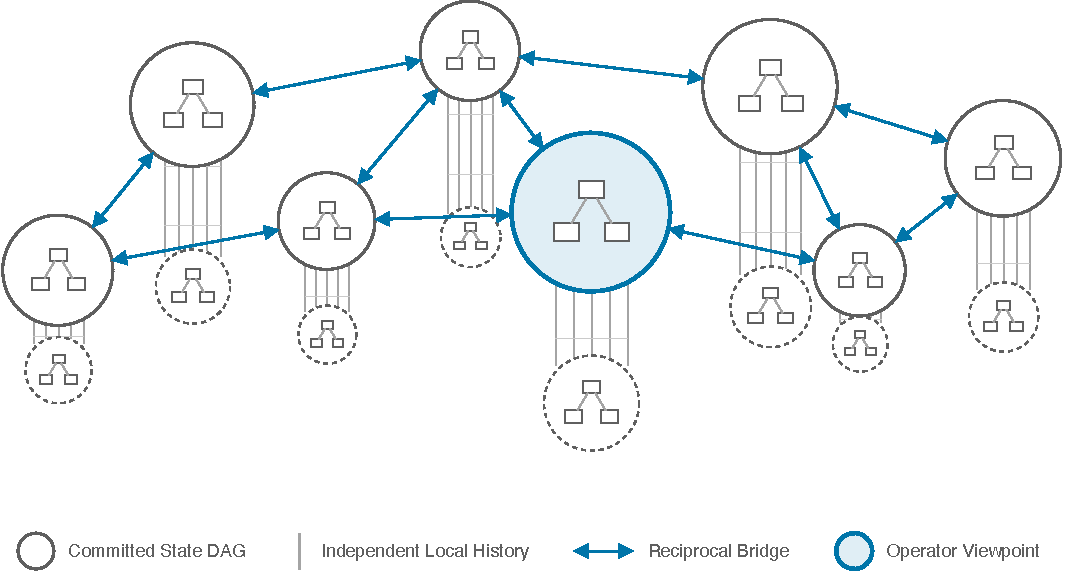
\includegraphics[scale=0.851]{figures/journal-relative-web.pdf}
  \caption{The Synchronic Web}
  \label{fig:journal-relative-web}
\end{figure}

\subsection{Scope and Lineage}

This paper is an architectural design and rationale. It describes the implemented integrity, history, object, and federation mechanisms and the assurance boundaries of their composition. The original Synchronic Web proposed a globally synchronized notary architecture~\cite{dinh2023synchronic}. The present design retains the name and broad aspiration but begins from independent journals, partially retained state, and sparse historical composition. Secure timelines and timeline entanglement supply the direct lineage for cross-history ordering~\cite{Maniatis2002timeline}. The architecture developed here asks what becomes possible when those histories carry everyday resources together with the definitions that interpret those resources.
\section{Integrity-Protected State}
\label{sec:integrity-state}

This section introduces the storage model on which the architecture rests. Any party holding a commitment can verify data against it, even when it holds only part of that data. \Cref{sec:history-entanglement,sec:self-encoding,sec:journal-web} each build on this model.

\subsection{The Value of Verifiable State}

Versioned systems preserve the path by which information changed. Git turns a working tree into a succession of content-addressed snapshots, append-only databases and blockchains bind later entries to earlier ones, and transparency systems publish authenticated views that clients and witnesses can compare~\cite{Haber1991timestamp,Laurie2014certificate,Melara2015coniks}. Their common achievement is to establish whether the evidence now presented belongs to the state that was previously committed. That answer changes the character of a \glslink{record}{record}. A mutable database row can only be read by asking the operator for its current value, whereas a committed state can also be held by a recipient, cited by \glslink{digest}{digest}, compared with another copy, and revisited after the operator changes its presentation. Recipients can preserve history alongside the service as portable evidence. This property remains valuable even when the record is incomplete, disputed, or false, because \glslink{integrity}{integrity} preserves the subject of later analysis rather than vouching for its truth.

Authenticated data structures typically deliver these guarantees through queries, in which a verifier receives a query result and a compact proof against a known root~\cite{Martel2004general,Miller2014authenticated}. This paper calls the property of being checkable against a commitment \emph{integrity-verifiable} and reserves \glslink{authentication}{authentication} for identity, origin, and authority, keeping digest consistency, signatures, and authorization visible as separate checks. The \glslink{synchronic-web}{Synchronic Web} departs from this query-and-proof model by making partial knowledge persistent, so that a recipient can retain one region of a state, discard another, and later combine compatible evidence while referring throughout to the same logical commitment. That capability begins with a deliberately small structural model.

\subsection{A Minimal Verifiable Structure}
\label{sec:minimal-structure}

The native substrate is an integrity-verifiable binary data-structure DAG in which immutable substructures may be shared by many parents. Uniform two-child nodes keep identifier derivation, slicing, and proofs the same everywhere, and richer structures such as maps and chains are built from them above the substrate. A \emph{logical digest} names recursively defined content or structure, while a \emph{node identifier} retrieves the representation available in one store. The separation matters because identity and storage answer different questions. The same logical state may use different persistence layouts, and one store may hold either complete structure or a compact record of its digest. A root is a \emph{durable handle}, a stable local name that maps to the node identifier of the current state, and branches, leaves, \glslink{stump}{stumps}, and null describe the structure reachable from a root. These concepts support maps, \glslink{object}{objects}, histories, and \glslink{resource}{resources}, as shown in \cref{fig:dag-stump}:

\begin{itemize}
  \item \textbf{Root:} a durable handle mapped to a \glslink{node}{node} identifier.
  \item \textbf{Branch:} two child node identifiers with a logical digest derived from their digests.
  \item \textbf{Leaf:} raw content bound into the structure by its digest.
  \item \textbf{Stump:} one retained digest for structure whose internal representation is unavailable.
  \item \textbf{Null:} the distinguished all-zero byte value denoting empty structure.
\end{itemize}

Each stored node is looked up by its node identifier, which also fixes the node's kind. A node's kind must be explicit, because a stump and the structure it replaces commit to the same digest; a store keyed by digest alone could not tell complete structure from a placeholder. Each kind consequently derives its identifier differently.\footnote{\Cref{fig:dag-stump} writes these derivations with $H$ for the hash function and $\|$ for concatenation.} A branch hashes its digest together with both child identifiers, a leaf uses its digest (the double hash of its content), and a stump hashes two concatenated copies of its digest. Null, by contrast, requires no stored record, since it is simply the all-zero byte value. Navigation from a record's durable handle thus never confuses one node kind with another. Because a digest commits recursively to everything beneath it, changing one leaf produces new digests along every dependent path to the root. The old node digest nonetheless continues to identify the old state, and advancing the root's durable handle selects its \glslink{successor}{successor}. Local mutation is therefore movement among immutable logical states.\footnote{In the Lisp layer of \cref{sec:lisp-structure}, branches appear as pairs, leaves as byte vectors, and stumps as stubs.}

\begin{figure}[htbp]
  \centering
  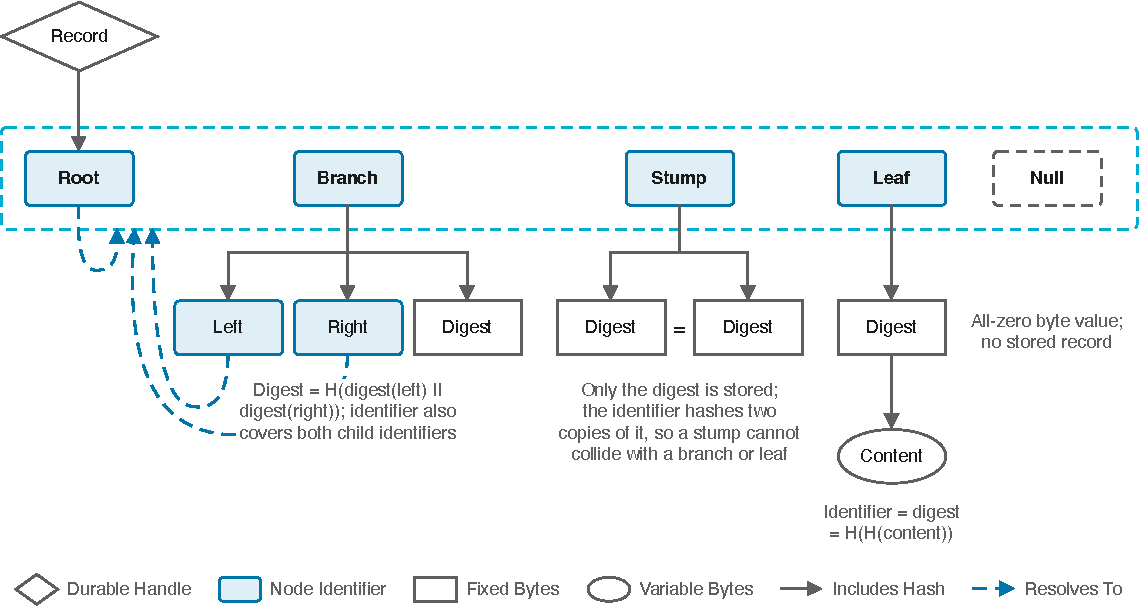
\includegraphics[scale=0.851]{figures/dag-stump.pdf}
  \caption{Roots and Partial State}
  \label{fig:dag-stump}
\end{figure}

\subsection{Proof Under Partial Knowledge}
\label{sec:partial-knowledge-proof}

The stump gives missing structure a precise place in this model by preserving the digest expected at one position and ending traversal at an identified boundary. Two states must remain distinct: null records actual emptiness, and a stump records committed structure awaiting evidence. A read that reaches a stump therefore returns a distinguished unknown value and makes no claim about what lies beneath. Partial knowledge is thus a precise statement about which regions of one immutable state are currently known.

Three operations move a state between levels of knowledge without changing its identity: slicing and pruning reduce the retained evidence, and merging restores missing evidence. A \glslink{slice}{slice} follows selected semantic \glslink{path}{paths} through a complete state and replaces unrelated material with stumps. Because the result retains the original root digest, every included resource remains bound to the complete state from which it came. Object-aware slicing follows compatible documented protocols as well as physical DAG edges. Object code may guide that traversal, but it is never trusted to preserve integrity, since the recipient verifies the resulting root against its accepted commitment. Slicing thereby extends the economy of compact Merkle multiproofs~\cite{Ramabaja2020compact}. A \glslink{journal}{journal} can apply the same stump replacement to material it already holds. \glslink{prune}{Pruning} shrinks what the journal retains and leaves the logical state, including every digest, unchanged. \glslink{merge}{Merge} moves in the other direction by replacing a stump with matching structure or recursively combining compatible branches. A digest mismatch aborts the operation, since the substrate cannot know which version a domain would prefer, and conflict resolution remains a matter of domain policy.

Partial states must also cross transport boundaries, and serialization carries node kinds, bytes, and retained digests between journals. A client can therefore reconstruct the same logical root, retain one proof, and accumulate neighboring evidence through later responses. \Cref{alg:deep-slice,alg:deep-prune,alg:merge-partial} give the slice, prune, and merge procedures. Each procedure evaluates the object it traverses (\cref{sec:objects}) and calls that object's operations.\footnote{Following Scheme convention, a name ending in \texttt{!} denotes an operation that modifies its target.}

\begin{algorithm}[htbp]
\caption{Deep Slice Along Object Path}
\label{alg:deep-slice}
\begin{algorithmic}[1]
\Require Object $x$ implementing digest-preserving slice/set protocols; nonempty available path $p$
\Ensure The selected path remains available and the logical digest remains fixed
\Function{DeepSlice}{$x,p$}
  \State $o \gets \texttt{sync-eval}(x)$
  \State $k \gets \Call{First}{p}$
  \If{$|p| = 1$}
    \State $o.\texttt{slice!}(k)$
    \State \Return $\Call{Node}{o}$
  \EndIf
  \State $c \gets o.\texttt{get}(k)$
  \State $d \gets \Call{Digest}{c}$
  \State $q \gets \Call{Rest}{p}$
  \State $c' \gets \Call{DeepSlice}{c,q}$
  \If{$\Call{Digest}{c'} \ne d$}
    \State \Call{Fail}{``slice changed child digest''}
  \EndIf
  \State $o.\texttt{set!}(k,c')$
  \State $o.\texttt{slice!}(k)$ \Comment{Discard siblings not needed for $k$.}
  \State \Return $\Call{Node}{o}$
\EndFunction
\end{algorithmic}
\end{algorithm}


\begin{algorithm}[htbp]
\caption{Deep Prune Along Object Path}
\label{alg:deep-prune}
\begin{algorithmic}[1]
\Require Object $x$ implementing digest-preserving prune/set protocols; nonempty path $p$ (may cross stumps)
\Ensure Evidence at the selected path is removed while the logical digest remains fixed
\Function{DeepPrune}{$x,p$}
  \State $o \gets \texttt{sync-eval}(x)$
  \State $k \gets \Call{First}{p}$
  \If{$|p| = 1$}
    \State $o.\texttt{prune!}(k)$
    \State \Return $\Call{Node}{o}$
  \EndIf
  \State $c \gets o.\texttt{get}(k)$
  \If{$c$ is not an available branch}
    \State \Return $\Call{Node}{o}$
  \EndIf
  \State $d \gets \Call{Digest}{c}$
  \State $q \gets \Call{Rest}{p}$
  \State $c' \gets \Call{DeepPrune}{c,q}$
  \If{$\Call{Digest}{c'} \ne d$}
    \State \Call{Fail}{``prune changed child digest''}
  \EndIf
  \If{$c'$ is a stump}
    \State $o.\texttt{prune!}(k)$
  \Else
    \State $o.\texttt{set!}(k,c')$
  \EndIf
  \State \Return $\Call{Node}{o}$
\EndFunction
\end{algorithmic}
\end{algorithm}


\begin{algorithm}[htbp]
\caption{Deep Merge of Compatible Structures}
\label{alg:merge-partial}
\begin{algorithmic}[1]
\Require Partial structures $a$ and $b$
\Ensure The result contains the union of available evidence and retains the common digest
\Function{MergePartial}{$a,b$}
  \If{$\Call{Digest}{a} \ne \Call{Digest}{b}$}
    \State \Call{Fail}{``cannot merge different digests''}
  \EndIf
  \If{$a$ is null}
    \State \Return $a$
  \ElsIf{$a$ is a leaf}
    \State \Return $a$
  \ElsIf{$a$ is a stump}
    \State \Return $b$
  \ElsIf{$b$ is a stump}
    \State \Return $a$
  \Else
    \State $a_L \gets \Call{Left}{a}$; $b_L \gets \Call{Left}{b}$
    \State $a_R \gets \Call{Right}{a}$; $b_R \gets \Call{Right}{b}$
    \State $l \gets \Call{MergePartial}{a_L,b_L}$
    \State $r \gets \Call{MergePartial}{a_R,b_R}$
    \State \Return $\Call{Branch}{l,r}$
  \EndIf
\EndFunction
\end{algorithmic}
\end{algorithm}


\subsection{Integrity as Infrastructure}

Partial knowledge separates auditability from bulk custody. An auditor need retain only the report, definitions, path, and ancestor evidence relevant to one decision, while the source keeps operational data in its native system. Another institution may preserve a complementary slice, and the two copies remain comparable because both resolve to the same commitment. Integrity does not, however, guarantee availability, which depends on institutions that replicate, \glslink{pin}{pin}, and renew media. A digest may outlive every full copy of the bytes it names. Integrity lets anyone check a recovered copy, but only retention determines whether recovery remains possible. When parties with different interests and storage budgets share these responsibilities, each can transfer, cite, sample, or inspect only the material it needs. The substrate is kept deliberately small because it concentrates trust, and everything above it is meaningful only if its primitives are correct. Rich semantics stay above it in stored objects, where they remain visible and can evolve historically. Structural validity alone is not a sufficient defense, since well-formed evidence may still be adversarially deep or broad; verification therefore also bounds how large, deep, and expensive an accepted proof may be. Within those bounds, the substrate adds verifiable internal partiality to content addressing, so that structure can be selectively retained and later restored under one identity. Signed committed \glslink{step}{steps} then extend that identity across change.

\section{History and Entanglement}
\label{sec:history-entanglement}

This section extends the verifiable state of \cref{sec:integrity-state} into a signed history of changes maintained by each \glslink{journal}{journal}. It also shows how independent organizations can link their histories so that each serves as evidence for the other, which \cref{sec:journal-web} later develops into access across the network.

\subsection{Connecting Independent Histories}

Organizations already exchange information through shared clouds, data lakes, APIs, replicated databases, signed documents, and ledgers. Each arrangement chooses a center of gravity, and each choice carries a corresponding limitation. A shared platform centralizes custody and policy, while replication multiplies copies of a single application state. Signed files travel independently but carry little context about succession, and webs of trust connect keys and attestations while leaving application data to other systems. Blockchain bridges transfer claims between consensus domains but inherit the complexity of both sides. However, many relationships do not cleanly fit any of these models. A manufacturer and buyer, laboratory and regulator, or publisher and archive each keep their own history, yet still need evidence that the other party's state existed before a later local event, even after the other party becomes unreachable. What is required, then, is a connection between histories that leaves each institution's governance intact. Secure timelines provide the starting point. A service repeatedly commits its state into a one-way succession, so later authenticators can establish the order of earlier states. Timeline \glslink{entanglement}{entanglement} carries signed authenticators across service boundaries and embeds them in other services' later authenticators~\cite{Maniatis2002timeline}. The embedding creates portable temporal mappings in which the past of one service becomes an input to the future of another. \glslink{synchronic-web}{Synchronic Web} \glslink{bridge}{bridges} apply that principle to histories whose states contain application \glslink{resource}{resources} and executable interpretation.

\subsection{Signed Local History}
\label{sec:signed-history}

Before journals can connect their histories, each must have a history to share. A journal builds it by turning local mutation into committed \glslink{step}{steps}. Applications accumulate a proposed state, inspect it, and then ask the journal to advance. The journal compares the proposal with the previous \glslink{head}{head} and stores transition metadata along with explicit inputs such as time and retained remote heads. It then binds its descriptor (the committed name, interface key, and endpoint through which others reach the journal) and key material into the new entry, constructs a canonical view of the chain with its signature fields blank, signs its \glslink{digest}{digest}, and advances the durable root. An authorized signing-key transition also requires a step, even when application state is unchanged, because the key that signs later heads is itself part of the committed history. Time, remote responses, randomness, and operator choices enter as explicit recorded values; anything the journal did not record cannot later be reproduced or verified. Applications that need exhaustive provenance, however, store event \glslink{object}{objects} or batch descriptions. \Cref{fig:step-anatomy} shows the logical result: application state, transition metadata, retained remote heads, time evidence, key-derivation and key-lineage material, and signatures share one integrity-protected tree built from the node structure of \cref{sec:minimal-structure}.\footnote{Reserved top-level names, marked with asterisks, separate application state (\texttt{*state*}) from journal-maintained structure.} \Cref{alg:commit-step} summarizes the commitment boundary: bind the \glslink{successor}{successor} state to its descriptors and any authorized key transition, sign the canonical view of the chain, and apply local retention policy without changing the logical history.

\begin{figure}[htbp]
  \centering
  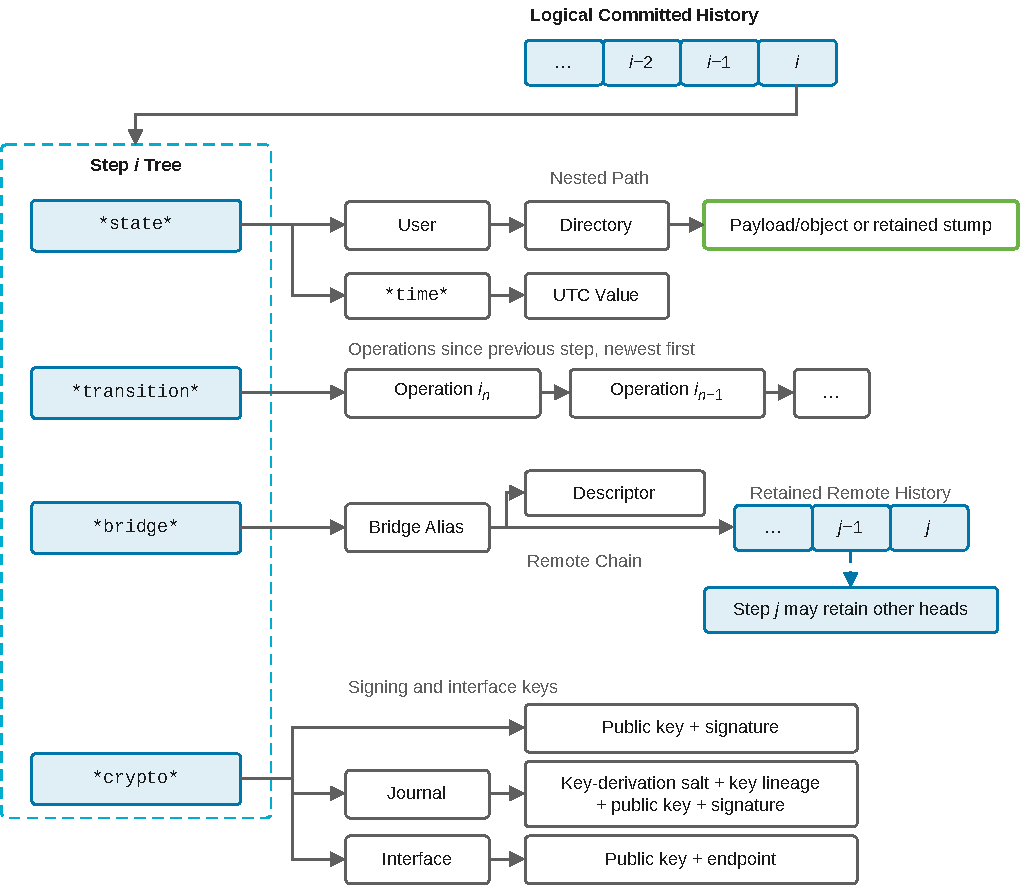
\includegraphics[scale=0.851]{figures/step-anatomy.pdf}
  \caption{Committed Step Anatomy}
  \label{fig:step-anatomy}
\end{figure}

\begin{algorithm}[htbp]
\caption{Commit Journal Step}
\label{alg:commit-step}
\begin{algorithmic}[1]
\Require Journal $J$, prepared time $t$, signing key pair $(p_k,s_k)$
\Ensure If state changed or a key transition is pending, a signed successor extends history and local retention is updated
\Function{CommitStep}{$J,t,p_k,s_k$}
  \State $(S,P,T) \gets \Call{JournalViews}{J}$ \Comment{Stage, permanent history, recent history.}
  \State $r \gets \Call{PendingKeyTransition}{J}$
  \State \Call{ValidateSigningContinuity}{$J,p_k,r$}
  \If{staged state is unchanged and no key transition is pending}
    \State \Return \Call{Size}{$P$}
  \EndIf
  \State $(S',H) \gets \Call{PrepareSuccessor}{S,t}$
  \State $C \gets \Call{Append}{P,H}$
  \State $C \gets \Call{BindDescriptorsAndKeyTransition}{C,J,r}$ \Comment{Written into the latest entry.}
  \State $C \gets \Call{BlankLatestSigningFields}{C}$
  \State $d \gets \Call{Digest}{\textproc{Node}(C)}$ \Comment{The enclosing chain is the signing object.}
  \State $\sigma \gets \Call{Sign}{s_k,d}$
  \State $P' \gets \Call{FillLatestSigningFields}{C,p_k,\sigma}$
  \State $(P',T') \gets \Call{ApplyRetentionPolicy}{J,P',T}$
  \Statex \Comment{Permanent: continuity, time, pins; recent: full state in window.}
  \State \Call{InstallSuccessor}{$J,S',P',T',r$}
  \State \Return \Call{Size}{$P'$}
\EndFunction
\end{algorithmic}
\end{algorithm}


Committed history grows without bound, so each journal must decide how much of it to keep. Historical identity and historical retention are separate choices, and keeping them separate is what makes long histories affordable. While a journal may retain recent heads in full, its permanent history keeps only chain continuity, signatures, selected proofs, and \glslink{pin}{pins}. \glslink{prune}{Pruning} replaces released material with \glslink{stump}{stumps}, using the partial-knowledge operations of \cref{sec:partial-knowledge-proof}. Pinning \glslink{merge}{merges} a chosen \glslink{slice}{slice} into the evidence held for a historical head, and unpinning releases that local obligation. A finite recent-history window therefore expresses a retention policy and makes no archival promise. Shrinking it immediately releases newly excluded unpinned material, while later widening changes future retention without reconstructing what was released. Each party preserves what serves its purpose and bears the cost of only that evidence. A buyer can pin an inspection report and its definitions, an archive can retain a complete site capture, and a witness can store signed heads and inclusion receipts. Related states share immutable structure, which reduces duplication, and replication and media renewal turn local retention into long-term availability.

\subsection{A Bridge Between Histories}
\label{sec:bridge-histories}

A bridge is a reciprocal signed-head-retention relationship. The journal that creates it becomes the sole ongoing synchronization initiator, and the acceptor returns its own signed head in the same exchange. Assigning that role to one side lets a private or intermittently reachable journal participate through outbound connections alone, while each journal keeps its commit cadence under local control. As shown in \cref{fig:bridge-reciprocal}, the initiator sends signed history and its descriptor under its current journal key. The acceptor verifies the sender's key lineage from its retained head, the committed endpoint, and that the new head extends the one already retained, before staging that head and returning corresponding evidence. The initiator performs the same checks locally, so neither side accepts evidence it has not verified itself. Each staged head enters the receiving journal's history at that journal's next local \texttt{step!}, and this inclusion orders the two histories. If B includes A's head $A_i$ in $B_j$, then $A_i$ precedes $B_j$, and $B_j$ with an inclusion proof serves as a portable receipt of that order. Because each journal commits on its own schedule, repeated exchange produces a weave of coarse ordering relations rather than a single global order, and each journal keeps its own sequence.

\begin{figure}[t]
  \centering
  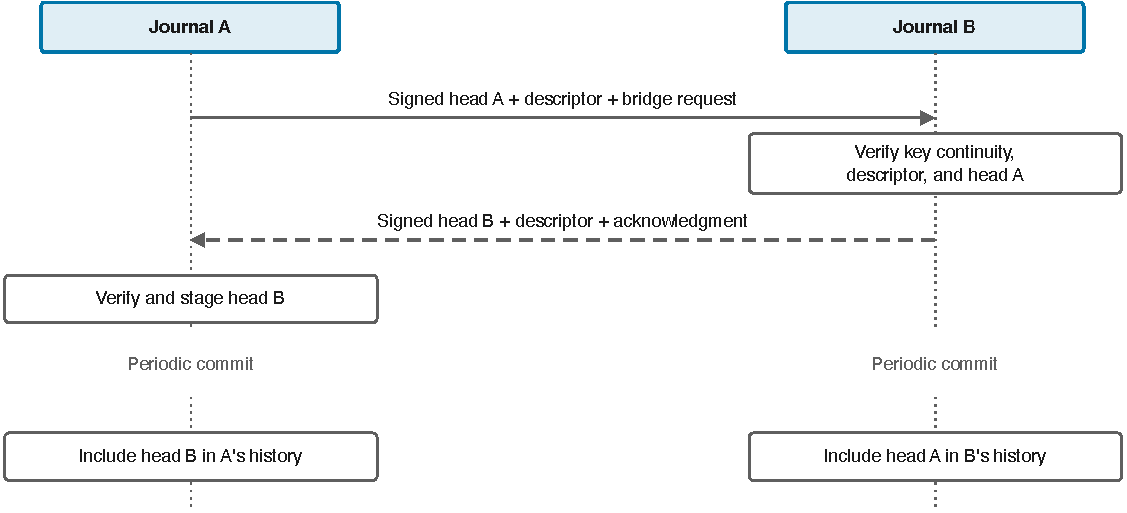
\includegraphics[scale=0.851]{figures/bridge-reciprocal-sequence.pdf}
  \caption{Bidirectional Head Exchange}
  \label{fig:bridge-reciprocal}
\end{figure}

Bridge operation also exposes practical controls. Synchronization cadence determines temporal resolution and network cost, and the bridge protocol determines the public material exchanged. Admission policy spans a range, from locked-down journals that accept incoming relationships only from preapproved signing keys, to open journals that may automatically accept any valid relationship.\footnote{Repeated synchronization safely confirms or advances acceptance, an already matching relationship can be re-checked read-only, and local stepping remains independent of remote traffic.}

\subsection{History at Network Scale}
\label{sec:network-history}

Sparse bridges turn entanglement into a network property. Because a remote head may itself contain other included heads, historical reachability composes recursively. From one selected journal, a verifier can follow retained heads across several relationships while preserving the path by which each piece of evidence became known. The result is a Web of historical viewpoints, each retaining its own timeline. This structure also governs how the network can grow. A ledger maintains one authoritative state for all participants, so every update that affects shared state must pass through a single consensus process and every full participant must process the updates of all others; the capacity of that consensus bounds the network~\cite{HarrisBraun2018holochain}. However, no single journal holds a globally authoritative state. Each is authoritative only for its own history and reaches agreement only with the journals it bridges, so its cost depends on its own activity and relationships rather than on the size of the network.

At this scale witnesses become central. A witness is any party, often another journal, that retains a journal's signed heads and compares them with the heads others received. Witnesses matter because nothing in the bridge protocol alone prevents a journal from signing distinct forks for journals that do not exchange evidence with each other. When witnesses compare heads or later histories include conflicting views, each journal retains the signed divergence as evidence. Transparency overlays and gossip develop this comparison as a general accountability technique~\cite{Chase2016transparency}. Each element plays a distinct role. Entangled journals contribute the retained remote heads, signatures establish authorship of each fork, and witness topology determines how quickly divergence becomes visible.

As these histories accumulate, object formats, \glslink{authorization}{authorization} rules, query languages, and application protocols will change on different schedules, and historical evidence remains most useful when the definitions needed to interpret it travel with the state itself. This change-management problem leads to the next layer, \glslink{self-encoding}{self-encoding} structure.

\section{Self-Encoding Structure}
\label{sec:self-encoding}

This section describes how the logic that interprets data is stored in the same verifiable structure as the data itself, using the substrate of \cref{sec:integrity-state} and the history of \cref{sec:history-entanglement}. Data and its interpretation can therefore be retained, transferred, and verified together.

\subsection{Code at Web Scale}

A durable network must survive software change as well as storage failure. Data written today may be read by another organization years later, after schemas, libraries, runtimes, and deployment practices have moved on. Preserving bytes answers only the first half of the archival question, because the reader also needs an account of how those bytes were structured and what operations gave them meaning. The Web already offers several partial approaches. JavaScript carries behavior to a widely available runtime, and Protocol Buffers and similar schema-driven encodings define stable wire forms and evolution rules whose schemas supply interpretation beyond each payload. Package managers and containers capture dependencies, while reproducible-build and software-transparency systems make artifacts traceable to declared sources and environments~\cite{Nikitin2017chainiac}. Each binds a different portion of the path from stored bits to behavior, but the data rarely carries that whole path. The gap matters because, at Web scale, change management crosses administrative boundaries. A recipient may accept data while declining the producer's newest software, or retain an old \glslink{object}{object} long after its originating service has migrated. Reproducibility also demands explicit treatment of time, randomness, network responses, and operator choices. \glslink{self-encoding}{Self-encoding} structure answers these pressures by placing a changeable definition inside the same commitment as the state it interprets. The resulting historical pair can travel, be sliced, and be cited together. The runtime consequently shrinks to a smaller shared foundation, application semantics become versioned material, and transitions can expose the environmental inputs on which their results depend.

\subsection{Lisp as Durable Structure}
\label{sec:lisp-structure}

Lisp gives code and data one inspectable representation. A method definition, query, path, transition, or configuration is an ordinary expression, so the network can hash, store, and transmit it like data and still evaluate it as code. This property, homoiconicity, is the reason for the choice of language. It turns semantic bootstrapping into structural composition, because the network can preserve the form describing an operation with the same substrate that preserves its inputs. The implemented runtime uses s7 Scheme~\cite{Schottstaedt2024s7} inside the \glslink{journal}{journal}. Native primitives provide the substrate of \cref{sec:integrity-state}, namely construction, hashing, persistence, \glslink{slice}{slicing}, network preparation, and controlled evaluation. Everything else, including maps, chains, signed histories, \glslink{authorization}{authorization}, and object protocols, is ordinary Scheme built above them. Because these structures are ordinary programs over the same primitives, applications can define others that favor different performance objectives, such as append-only commitments that give recently added items shorter membership proofs~\cite{Cevallos2025merkle}. The approach follows the tier-unifying intuition of single-language Web systems~\cite{Cooper2007links}, preserving explicit boundaries while reducing translations between stored state and application logic. The bootstrap terminates in native storage and evaluator semantics, which define how expressions are read, \glslink{node}{nodes} are hashed, and capabilities are exposed. Keeping this foundation small makes it practical to inspect and reproduce, and every higher layer can evolve as identified structure in journal history.

Within one language, objects may implement different methods and evolve under different authorities, yet remain transportable through the same node and evaluator model. Documented public behavior provides compatibility across class systems. Confinement is necessary because portable definitions arrive from parties who may use different software and policy. The implemented \texttt{sync-let} boundary copies inputs as plain data into a reduced environment of approved primitives, excludes direct access to the journal, network, time, randomness, and host, and copies results back to the caller as plain data. Finer per-object capability assignment is an optional extension that portable execution does not require. Capability confinement and evaluator isolation address different failures, continuing the distinction between restricted execution environments and other approaches to program safety such as proof-carrying code~\cite{Levy1995safe,Necula1997proof} and object-capability systems~\cite{LemmerWebber2025spritely}. While the evaluator isolates shared computation from host authority, the trusted host still controls persistence, networking, and consumption of compute and storage. Preserving an executable definition does not remove this dependency, because interpreting it still requires compatible evaluator semantics and a trusted execution boundary.

\subsection{Self-Encoding Objects}
\label{sec:objects}

A standard object is a node with executable definition on the left and state on the right. Its \glslink{digest}{digest} commits to both components and to their association. Evaluating that node with \texttt{sync-eval} produces a transient callable object. A zero-argument call returns its current node, documented method dispatch exposes behavior, and object-specific \glslink{path}{paths} expose state according to the object's protocol. \Cref{fig:self-encoding-transition} follows one transition as definition $D_0$ and state $S_0$ enter a controlled runtime with explicit input arguments, producing a candidate with revised definition $D_1$ and \glslink{successor}{successor} state $S_1$. However, evaluation alone changes nothing durable, since an authorized boundary chooses whether to persist that result. Because the starting object remains independently identifiable, semantic change takes the form of historical succession instead of replacement.

\begin{figure}[htbp]
  \centering
  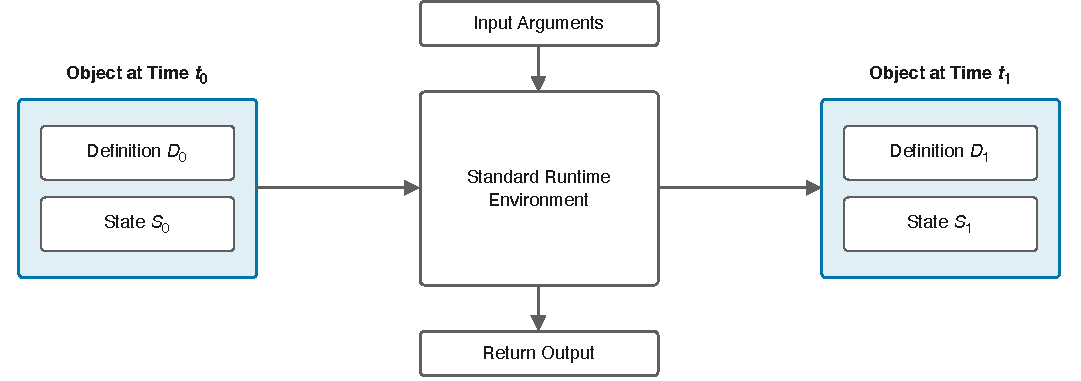
\includegraphics[scale=0.851]{figures/self-encoding-transition.pdf}
  \caption{Self-Encoding Object Transition}
  \label{fig:self-encoding-transition}
\end{figure}

Live and durable mutation are deliberately separate and meet only at explicit persistence. A method may update the live object's state, but the change becomes history only when the journal extracts the new node and stores it into its parent or root. Nested mutation follows the same rule along the return path, where each containing object is rebuilt in turn, every predecessor remains available by digest, and the durable boundary stays visible in code. Objects compose through public protocols, so deep reads can traverse semantic boundaries while deep mutations rebuild ancestors. Deep slicing and \glslink{prune}{pruning} ask each object to retain evidence appropriate to its layout, and deep \glslink{merge}{merge} restores compatible partial material under matching commitments. \Cref{tab:deep-operations} summarizes this implemented family. The caller places shared computation inside the confinement boundary of \cref{sec:lisp-structure} before loading an object with \texttt{sync-eval}, so environmental values reach untrusted code only as copied data. Authorization and storage then turn the candidate result into history.

\begin{table}[htbp]
  \centering
  \small
  \begin{tabularx}{\textwidth}{@{}>{\ttfamily\frenchspacing}P{0.125\textwidth}>{\ttfamily\frenchspacing}P{0.38\textwidth}X@{}}
\toprule
\normalfont\textbf{Operation} & \normalfont\textbf{Signature} & \textbf{Behavior} \\
\midrule
deep-get    & (deep-get object path) & Traverse nested public \texttt{get} methods and return the value at the path. \\
deep-set!   & (deep-set! object path value) & Set the terminal value and rebuild each ancestor. \\
deep-slice! & (deep-slice! object path) & Retain evidence along the path while preserving the logical digest. \\
deep-prune! & (deep-prune! object path) & Remove path evidence, rebuilding parents or replacing exhausted children with stumps. \\
deep-merge! & (deep-merge! source target path) & Merge digest-compatible evidence into the target or into the optional target path. \\
deep-copy!  & (deep-copy! object source target) & Copy the value at one nested path to another. \\
deep-call   & (deep-call object path callback) & Evaluate a callback against the selected object and return its result, leaving ancestors unchanged. \\
deep-call!  & (deep-call! object path callback) & Evaluate once and return the result with the complete rebuilt root. \\
\bottomrule
\end{tabularx}

  \caption{Deep Object Operations}
  \label{tab:deep-operations}
\end{table}

\subsection{Shared Computation in Practice}
\label{sec:shared-computation}

Beyond individual objects, the journal supports several forms of shared computation. The standard object library grows semantics from a small evaluator. Portable classes compose through public protocols, journals place results into signed history, and application-defined objects carry domain concepts. Stored programs use a journal capability to compose standard journal operations, including historical resolution and retention, in the native path, history, and object vocabulary.\footnote{An administrator may also configure one stored program to launch after each successful commit, receiving that commit's index. The launch is best-effort and periodic, since launches may overlap and a process failure after commit can lose a launch.} Historical \texttt{retrieve} can also exercise an object method without persisting its successor. The requesting journal checks the returned proof against the selected commitment and recomputes the result using the definition and state in the proof. These facilities extend the substrate under three controls:

\begin{itemize}[nosep]
  \item \textbf{Deterministic object evaluation.} A confined object's candidate successor derives from its definition, starting state, explicit arguments, compatible evaluator semantics, and controlled primitives. Multi-call stored programs may observe changing journal state and are therefore not fully replayable.
  \item \textbf{Resource governance.} Execution bounds constrain a single operation and its descendants, but aggregate resource exhaustion still requires host-level admission control. Failure discards an uncommitted candidate but does not undo previously completed nested journal operations.
  \item \textbf{Explicit evolution.} Public protocols and layouts are compatibility contracts. Migrations must state authority, validation, rollback, partial-object behavior, and runtime compatibility rather than treating executable history as automatic semantic compatibility.
\end{itemize}

These controls together keep shared computation reproducible where it matters and leave its operational limits to host policy.
\section{The Journal-Relative Web}
\label{sec:journal-web}

This section combines the state, history, and interpretation layers of \cref{sec:integrity-state,sec:history-entanglement,sec:self-encoding} into a Web in which each \glslink{journal}{journal} serves as its own point of reference. It describes how resources are named, accessed across organizational boundaries, and governed by local rules.

\subsection{A Web of Resources}

The conventional Web organizes interaction around sites, origins, URLs, \glslink{resource}{resources}, representations, links, and clients~\cite{Jacobs2004webarch,BernersLee2005uri}, and the \glslink{synchronic-web}{Synchronic Web} gives each term a historical counterpart. A journal resembles a site with its own administration and evolving state. Its root supplies an origin for interpretation, a \glslink{path}{path} identifies a resource from that root, and a committed \glslink{head}{head} selects the historical view in which resolution occurs. The returned representation may be bytes, an expression, a partial proof, or a \glslink{self-encoding}{self-encoding} \glslink{object}{object}. A path such as \texttt{(*state* components c17 inspection)} lists segments from the journal root, like a filesystem path, where \texttt{*state*} names the application namespace and the remaining segments select nested resources. Such a path gives a resource continuity across versions, while a \glslink{digest}{digest} identifies the exact state found there at one head. A client can therefore request the current resource, resolve the same path at an earlier \glslink{index}{index}, or cite one particular representation by digest. Paths cross semantic as well as structural boundaries, and one segment may enter a tree, another an object, and another a remote history retained beneath a \glslink{bridge}{bridge} (\cref{sec:network-history}). Each object interprets its documented portion, and end-to-end evidence is preserved across every boundary. Because historical states remain addressable, ordinary links embedded in representations can cite a persistent version rather than only a moving current resource. Relative references remain ordinary URI references interpreted by the client against the selected resource~\cite{Rivest1996sdsi,Mazieres1998path}.

Every journal thus induces a distinct coordinate system over local and remote state. A bridge segment encodes the relationship through which remote state became reachable, a historical index selects the committed viewpoint, and content-derived identifiers name exact representations~\cite{Haber1997secure,Kuhn2014trusty,Zhang2014named}. The practical consequence is that a prior state joins the same address space as the current one. Partial evidence can travel as its representation, and clients can distinguish unknown structure, empty structure, unavailable data, policy denial, and unreachable endpoints.\footnote{A committed read can return the absolute local and per-hop indexes selected by that same operation through optional index metadata, so the client can turn a current-head selection into a fixed historical reference.}

\subsection{Access Across the Web}
\label{sec:access-paths}

A path names a resource relative to the journal that resolves it, and the same form extends across bridges. The canonical public form is one flat journal-relative path: an index at the origin journal, then each directional bridge alias followed by a destination index, then a namespace and a local path interpreted at the destination journal. Thus \texttt{(20 carol 15 bob -3 *state* docs report)} selects a historical index at every journal, and negative indexes count back from the latest, so \texttt{-1} selects the current head and \texttt{-3} the head two steps earlier. The alias-and-index prefix is the path's \glslink{route}{\emph{route}}, the sequence of journal-to-journal bridge hops that reaches the destination. Aliases are receiver-local names with no global meaning, and indexes may be omitted when current. Live \texttt{put!}, \texttt{use!}, and \texttt{copy!} follow the current committed object at each hop. \texttt{retrieve} instead combines that current route for \glslink{authentication}{authentication} and endpoint context with independently selected historical indexes for content. Returned evidence may fill a \glslink{stump}{stump} only when its digest remains fixed. A route never advances an embedded remote head to a newer one; each hop uses the exact state committed beneath its parent, which is what allows every hop of the route to be verified against evidence the origin already holds.

\Cref{fig:federated-invocation} shows the exact-object handshake and direct invocation at the destination:

\begin{itemize}
  \item \textbf{Exact forward route.} From A's selected committed head, each hop follows the nested journal object already stored there, through intermediate journal B, until A reaches the exact C object containing C's interface signing key, endpoint, and index/digest context.
  \item \textbf{Receiver-relative return.} C returns a partial object at that same historical C head containing C's reverse route to A's interface key. A requires its index, digest, and reverse sequence to agree with the C object already committed beneath A's forward route~\cite{dinh2025identity}.
  \item \textbf{Direct application call.} A signs and sends the C object with the resource invocation directly to the committed canonical endpoint.\footnote{Intended production deployments use HTTPS.} C matches the raw supplied-object digest against its own history before evaluation, reconstructs the bridge \glslink{principal}{principal} that names A, checks the signature against the key reached by the reverse route, and authorizes the request locally. Intermediaries see public route/control metadata, while the private function, path, arguments, and value travel only on the final connection.
  \item \textbf{Result and retention.} Live invocation results receive only operational assurance, from the direct connection to the committed endpoint. \texttt{retrieve} additionally returns proof that A verifies against the selected historical C object. A may then retain that proof locally with a separate \texttt{pin!} over the full origin-relative historical path.
\end{itemize}

Invocations normally reach the attributed source in this way, but when that source is unavailable or should not be contacted, a client can instead select a retained responder. The responder interprets the requested history locally and serves only permanently retained evidence under its usual \glslink{authorization}{authorization}, resolving current-head selections against what it actually holds and reporting which indexes it retains. The origin anchors the proof to the responder's exact authenticated object and independently derives those selections before verifying the content. \Cref{tab:resource-operations} groups the public resource operations by architectural purpose.


\begin{figure}[htbp]
  \centering
  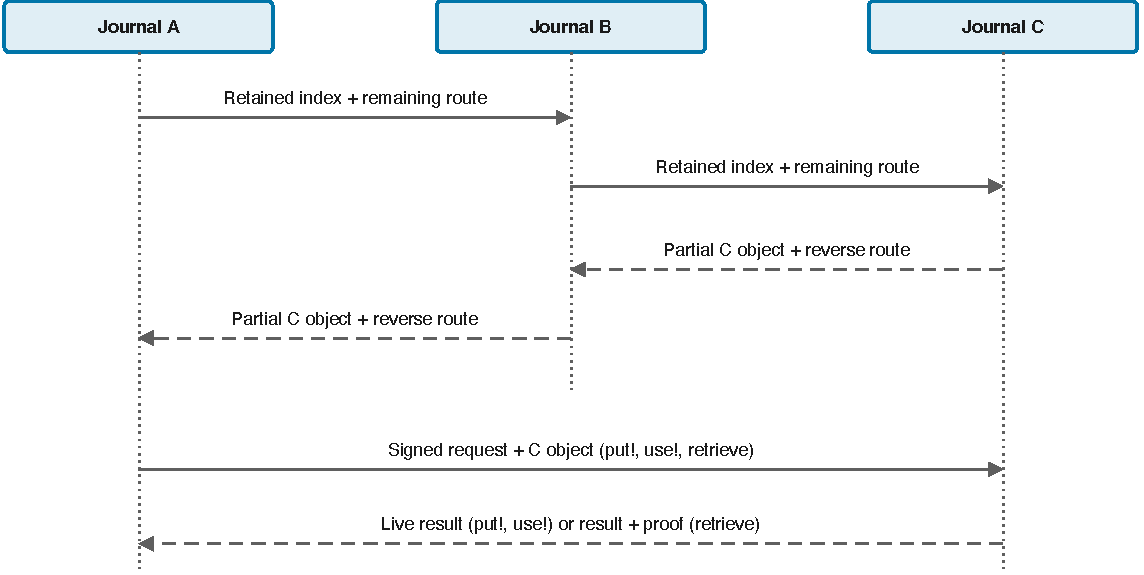
\includegraphics[scale=0.851]{figures/federated-invocation-sequence.pdf}
  \caption{Exact-Object Route and Invocation}
  \label{fig:federated-invocation}
\end{figure}

\begin{table}[htbp]
  \centering
  \small
  \begin{tabularx}{\textwidth}{@{}P{0.25\textwidth}P{0.285\textwidth}X@{}}
\toprule
\textbf{Purpose} & \textbf{Operations} & \textbf{Architectural Boundary} \\
\midrule
Store and copy & \texttt{put!}, \texttt{put-batch!}, \texttt{copy!}, \texttt{copy-batch!} & Change staged state, including deletion. Copy reads sources from one pre-mutation snapshot. \\
Exercise current objects & \texttt{use!}, \texttt{use-batch!} & Invoke objects, persisting successors atomically or discarding them in read-only mode. \\
Compose live operations & \texttt{run!} & Execute a stored program through a caller-bound journal capability. Nested calls keep their own authorization and mutation boundaries; the whole program is not atomic. \\
Retrieve historical evidence & \texttt{retrieve}, \texttt{retrieve-batch} & Read selected committed state or compute an object result from that state, verifying returned evidence without persisting successors. \\
Retain or release evidence & \texttt{pin!}, \texttt{pin-batch!}, \texttt{unpin!}, \texttt{unpin-batch!}, \texttt{prune!}, \texttt{prune-batch!}, \texttt{truncate!} & Change local retention without changing the selected historical commitments; authority and protected-path constraints remain local. Administrator-only truncation releases history through an index while preserving chain identity and numbering. \\
\bottomrule
\end{tabularx}

  \caption{Public Resource Operations}
  \label{tab:resource-operations}
\end{table}

\subsection{Keys and Principals as History}
\label{sec:keys-principals}

\glslink{integrity}{Integrity}, key continuity, and authorization form a continuous historical path, beginning with the key continuity checked at each bridge (\cref{sec:bridge-histories}). Bridge aliases serve as authorization principals whose meaning is local to the receiver. After a relationship is deleted, the same alias may name a different journal, so authorization rules attach to the receiver's naming choices rather than to any remote identity. The same verified committed head binds the journal name, interface key, and canonical endpoint. Routes therefore act as a decentralized public-key infrastructure bootstrapped from local trust. Each hop binds a remote journal's key and endpoint to a head the previous journal already committed, so a journal can discover and verify keys well beyond its direct bridges without any certificate authority. Unlike a conventional PKI, the resulting bindings are receiver-relative and only as current as the heads along the route. The journal signing key signs heads, whereas the interface key authenticates invocations, so the key used for requests can change without altering how history is signed. Because the keys are independent, compromise of the interface key exposes invocation authority without permitting the attacker to sign history. Compromise of the journal key, by contrast, permits forks, as described in \cref{sec:control-evidence}.

For an invocation, the origin supplies an explicit caller identity---its journal, a locally authenticated user, or a public caller---which the exact route turns into a receiver-relative principal such as \texttt{(dave erin *state* frank)}, which names user \texttt{frank} at the journal reached back through bridge aliases \texttt{dave} and \texttt{erin}. The destination also records which of its own history indexes held the committed bridge object that authenticated the origin key. An authorization rule can therefore require that key to have been confirmed recently in the destination's own history, a local bound on key age rather than a freshness guarantee about the request. The destination's rules grant path-scoped permissions separately for each operation class in \cref{tab:resource-operations}. Signed batches bind the ordered requests and any expected values, and the destination authorizes every member before mutation, so a batch cannot carry an unauthorized request alongside permitted ones. Conditional writes require both observation and mutation authority. Although finite routes may revisit a journal, the destination's authorization decides whether the resulting principal is permitted. Permission to read or invoke an object does not imply permission to run stored programs, and nested operations preserve and recheck the original caller so that indirection cannot widen authority.

Administrators are local principals with default execution authority, and all administrative operations---bridge management, configuration, authorization, and retention---remain local. Retention in particular never rewrites the committed state it describes (\cref{sec:partial-knowledge-proof}). Removing data therefore takes two steps. A \texttt{put!} of the empty value commits a successor state without the resource, and pruning the earlier states then releases their stored copies while preserving each historical commitment~\cite{Crosby2009efficient}. Bridge establishment similarly separates remote evidence gathering from atomic local mutation, so network interaction does not become an implicit distributed transaction. Signed requests, however, carry no freshness token, so a request may be replayed. \texttt{put!} keeps ordinary repeatable-write semantics, transport retries may repeat it, and applications add identifiers, idempotency, or state preconditions as their domain requires. Across all cases, the committed route identifies the origin, its signature authenticates the invocation and optional user attestation, and the destination's state maps the resulting principal to permitted operations.

\subsection{A Web of Viewpoints}

A mature Synchronic Web begins from the journal a person, organization, or application chooses to trust locally. That journal is simultaneously a store, historical memory, policy engine, and gateway into other histories. Following a link is a client action from this viewpoint, and the client resolves the target through the same historical addressing and local policy as any other resource. Discovery supplies candidate journals, endpoints, resources, and routes from any available source, whether descriptors, search services, existing links, or out-of-band knowledge. Historical continuity lets candidates update endpoints and interface keys and still preserve identity. Whatever their source, candidates become bridges or trusted routes only through local policy, and the journal's graph gradually records both reachable resources and the relationships through which they became meaningful.

Reachable resources also include state that originates outside any journal. Most useful data begins in operational systems, outside the addressable network form, and \cref{tab:data-forms} compares the strengths of each. A Web projection connects the two by mapping selected operational state into journal resources under a contract covering deterministic encoding, resource boundaries, correction, and deletion. The source can remain the system of record while an asynchronous projection supplies historical evidence, and mature clients may gradually let selected projected resources assume an operational role. Once projected, state becomes reachable through the same local paths and routes as any other resource (\cref{sec:access-paths}).

\begin{table}[htbp]
  \centering
  \small
  \begin{tabularx}{\textwidth}{@{}P{0.18\textwidth}XX@{}}
\toprule
\textbf{Aspect} & \textbf{Addressable Network Form} & \textbf{Query-Optimized Operational Form} \\
\midrule
Primary unit & Resources and relationships, each independently identified & Record, row, object, index, or transaction \\
Identity & Root-relative path plus the commitment of the resolved state & Application key interpreted within one operational system \\
Strengths & Linking, citation, selective transfer, plural ownership, and historical reference & Locality, transactions, compression, indexing, and efficient bounded queries \\
History & Resource states and cross-history relationships are first-class & Commonly application-defined, compacted, or maintained in separate logs \\
Typical costs & Traversal, synchronization, repeated metadata, and derived indexing & Provider dependence, schema coupling, and application-specific portability \\
Architectural role & Shared network projection and retained historical evidence & System of record and rebuildable derived views \\
\bottomrule
\end{tabularx}

  \caption{Complementary Data Forms}
  \label{tab:data-forms}
\end{table}

Clients are what make the architecture usable. A browser, filesystem, gateway, projection worker, or inspection tool chooses roots and heads, fetches and \glslink{merge}{merges} evidence, invokes objects, enforces policy, and applies retention intent. Routine interactions present plain resources, while audit views expose paths, signatures, \glslink{slice}{slices}, and receipts. Application vocabularies such as W3C PROV, domain schemas, scientific objects, and future protocols remain resources above the generic history and integrity layers~\cite{Moreau2010open,Moreau2013prov}. Their definitions evolve through self-encoding objects, and their relationships can identify resources across journal boundaries. The governing principle is that every resource is reached from a chosen viewpoint, every historical claim carries its evidence, and every act of trust belongs to the relying journal.
\section{Example Application Scenarios}
\label{sec:applications}

This section applies the design to four scenarios: Web archives, manufacturing traceability, digital identity, and reputation for automated agents. Each is a design exercise grounded in the implemented system, and none describes a deployed application. In every scenario, existing operational systems keep their current role, and the architecture adds value where several of its properties meet in the same resource.

\subsection{Decentralized Web Archives}

Web content changes and disappears, and today's archives preserve it as captures held by individual institutions. A conventional site can continue serving pages from its content system, and a projection worker gives selected \glslink{resource}{resources} journal-relative \glslink{path}{paths}. Each capture stores its deterministic representation, interpretation metadata, source path, and projection progress. While the site's current page remains convenient for browsing, the projected resource adds a history that independent archives can retain and verify. No single archive, however, need hold everything. Several may preserve overlapping portions of that history---one holding complete captures, another text and metadata, and a third selected high-value resources---and their \glslink{slice}{slices} remain comparable through shared commitments. Reciprocal \glslink{bridge}{bridges} can then place important source and archive \glslink{head}{heads} into one another's later histories. The resulting inclusion receipts survive the loss of any one service when another custodian retains the required evidence. A client whose \glslink{journal}{journal} can reach such an archive through bridges can select it as the retained responder, which serves only evidence it permanently retains, and verify the returned proof against the archive's authenticated object without contacting the vanished publisher.

Adoption can also proceed gradually, because nothing in the model requires existing systems to change. Static sites, databases, and content-management systems remain operational, and the projection adds an audit path. Native clients can later resolve historical resources directly, follow links into retained versions, or compare captures from several archival viewpoints. Even so, long-term operation demands capture-fidelity policy, privacy review, legal-erasure procedures, malicious-content handling, media renewal, and cryptographic migration~\cite{Chun2009tiered}, and the journal gives those activities a stable structure of record.

\subsection{Production Traceability}

Consider a manufacturer that stores an inspection report for component c17 in its quality-management database. A projection worker encodes the report at \texttt{(*state* components c17 inspection)}, where the path names the continuing production resource and an application-defined \glslink{object}{object} binds this version's bytes, metadata, and interpretation. The manufacturer's journal then commits the \glslink{successor}{successor} state as a new signed head. The projection extends existing traceability models with independently retained history~\cite{Stouffer2022traceability,Hasan2009provenance}. When a buyer requests evidence, the manufacturer slices that head along the inspection path, retaining the report, its definition, and the ancestor digests needed to verify the root. The buyer can \glslink{merge}{merge} and \glslink{pin}{pin} the slice under its procurement policy, while the manufacturer remains free to \glslink{prune}{prune} its own historical copy. If the two maintain a reciprocal bridge, the buyer also includes the manufacturer's head in a later head of its own, and the resulting inclusion proof serves as a receipt that the inspection state preceded the buyer's subsequent history (\cref{sec:bridge-histories}). Protected details travel separately through the exact-object \glslink{route}{route} of \cref{sec:access-paths}, under the manufacturer's own \glslink{authorization}{authorization}. The buyer therefore holds a proof it can present to an auditor or regulator without the manufacturer's further cooperation. A later correction appears as an identifiable successor rather than an overwrite, and the buyer can record acceptance, dispute, or follow-up inspection in its own history. Cryptographic evidence preserves the reports and their ordering, while physical identifiers, inspection practice, and institutional judgment connect that evidence to the component itself.

\subsection{Self-Sovereign Identity Anchors}

Online identities today typically live inside platforms and identity providers, so an account's name, connections, and history remain with the service where they accumulated. A person or organization can instead establish a stable path beneath a selected well-known root and use it as an anchor for a profile hosted by an evolving journal. The profile can contain current endpoints, public keys, service relationships, and links to selected claims, all interpreted by observers from roots they already recognize. Changing providers is then a historical transition, in which the earlier state points toward the successor relationship, the new host publishes its descriptor and key, and observers follow the retained trail according to their own policy. Historical resolution makes that trail concrete. Resolving the anchor path at an earlier index shows the profile as it stood before a change, and its \glslink{digest}{digest} cites that exact version. Key rotation is itself a committed step authorized by the predecessor key, so an observer can check each transition from the head it already retains (\cref{sec:bridge-histories}). While historic name trails developed a close model for changing personal online identifiers~\cite{Maniatis2003hints}, journal history extends the trail to richer state, reciprocal receipts, and application-defined relationships. Anchor operators, witnesses, and communities define how recovery, delegation, impersonation disputes, privacy, and endpoint discovery work. The journal structure leaves these questions to those rules and preserves the evidence they consume: prior keys, authorized transitions, witnessed heads, and competing forks. A person can change hosts while keeping the history through which others recognize the change.

\subsection{Agent Reputation Discovery}

A user can begin from journals and communities already trusted for a task, then follow committed relationships to reporting agents whose reports cite sources, record methods, receive corrections, and accumulate later outcomes. Reputation is therefore computed rather than assigned, because each user's journal derives it as a view under local rules, from inspectable history that can travel across ranking services. Different communities may retain different evidence and value prediction calibration, source transparency, or specialized performance, so their judgments can diverge while still citing common reports and outcomes. Secure per-node logs and deterministic replay offer a related accountability model~\cite{Haeberlen2007peerreview}, and partial journal history makes selected evidence portable across evaluators. Historical \glslink{integrity}{integrity} contributes stable inputs---which claim appeared, which sources accompanied it, which correction followed, and which community endorsed the result---that a chosen journal can combine into a local discovery view and preserve for inspection.

Automated agents make this model both more necessary and more practical. For people, digital \glslink{record}{records} largely reflect a physical world that offers independent checks such as personal acquaintance, institutional standing, and direct observation, whereas for an agent the digital record is the world itself, so the evidence behind its judgments has no external fallback. People typically rely on a platform to condense reputation into a score, since reading the underlying history at scale is impractical, and the method of condensation is rarely portable or open to inspection. Agents face no such constraint. They can read cited reports, sources, and corrections directly, and a reputation rule can be an ordinary \glslink{self-encoding}{self-encoding} object stored in an agent's own journal. Such a rule behaves like any other resource and can be versioned, cited, shared with other agents, and evaluated by any adopter against the same retained evidence. Because the rule is an object, another agent can retrieve it from a historical head and recompute its result from the definition and state in the proof (\cref{sec:shared-computation}) instead of trusting a reported score. Reputation thereby becomes a set of competing, inspectable definitions rather than a single opaque score, and an agent can refine its rule as outcomes accumulate without depending on a ranking service.

\section{Related Work and Lineage}
\label{sec:related-work}

This section compares the design with the research it draws on. It identifies what the design adopts from each line of work and where it departs, without attempting a complete survey. Nearly every ingredient has a substantial precedent, and the contribution lies in their composition, which develops earlier composable-ledger work~\cite{dinh2023composable} into a plural Web of partially retained, self-encoding state connected by entangled histories and journal-relative paths.

\subsection{Integrity and Entangled History}

Cryptographic timestamping establishes one-way succession among committed documents~\cite{Haber1991timestamp}. Persistent authenticated dictionaries make earlier versions queryable~\cite{Anagnostopoulos2001persistent}, and general authenticated-structure models and generic programming techniques extend the pattern across data structures~\cite{Martel2004general,Miller2014authenticated}. Compact multiproofs reduce repeated Merkle evidence, and tamper-evident logs organize efficient historical queries and controlled deletion~\cite{Ramabaja2020compact,Crosby2009efficient}. Transparency systems turn these structures toward public accountability. Certificate Transparency, CONIKS, and CHAINIAC use append-only or collectively witnessed histories to make authority behavior inspectable~\cite{Laurie2014certificate,Melara2015coniks,Nikitin2017chainiac}. PeerReview combines attributable logs with deterministic replay for distributed systems, and transparency overlays generalize witness comparison across applications~\cite{Haeberlen2007peerreview,Chase2016transparency}. Of this lineage, Maniatis and Baker's secure timeline \glslink{entanglement}{entanglement} is the most direct precedent for bridge-composed history~\cite{Maniatis2002timeline}. Timeweave imports signed threads from other timelines into later authenticators, yielding temporal mappings, inclusion receipts, and proofs that survive the originating service. Where Timeweave entangles service timelines, \glslink{synchronic-web}{Synchronic Web} \glslink{bridge}{bridges} carry this mechanism into sparse relationships among \glslink{journal}{journals} whose histories contain path-addressed, partially retained, \glslink{self-encoding}{self-encoding} state.

\subsection{Provenance and Preservation}

Untrusted-storage systems show how clients can retain compact state and detect server equivocation or tampering~\cite{Li2004secure,Mahajan2010depot,Kim2015caelus}. The Synchronic Web adopts the same client-held-commitment discipline but lets each journal maintain its own state and history. Database provenance distinguishes why- and where-provenance, while Web provenance models processes, evidence, and responsibility~\cite{Buneman2001why,Moreau2010foundations,Moreau2010open}. W3C PROV standardizes entities, activities, agents, derivations, and responsibility for interoperable exchange~\cite{Moreau2013prov}. Nanopublications package scientific assertions with provenance and publication context~\cite{Groth2010anatomy}, and secure provenance protects provenance \glslink{record}{records} as they cross untrusted environments~\cite{Hasan2009provenance}. These models complement the architecture, since they can inhabit journal \glslink{resource}{resources} as application vocabularies. Content-derived naming and distributed preservation supply another lineage. IPFS, Trusty URIs, secure names, and self-certifying paths bind identifiers to content or cryptographic authority~\cite{Benet2014ipfs,Kuhn2014trusty,Haber1997secure,Mazieres1998path}. Merkle-CRDTs use Merkle DAGs for convergent replication of conflict-free replicated data types (CRDTs), Named Data Networking centers retrieval on named data, and LOCKSS combines peer replication with auditing for preservation~\cite{Sanjuan2020merkle,Zhang2014named,Maniatis2005lockss}. Tiered fault tolerance treats rare failures and cryptographic aging as ordinary long-horizon events~\cite{Chun2009tiered}. The Synchronic Web joins these concerns through resources whose content, history, and interpretation can be retained at different levels of completeness.

\subsection{Decentralized Webs and Identity}

Web architecture separates resource identification, representations, and interaction, and RFC~3986 supplies global URI syntax and relative-reference resolution~\cite{Jacobs2004webarch,BernersLee2005uri}. While Memento adds datetime negotiation and TimeMaps for earlier resource states~\cite{VanDeSompel2013memento}, Synchronic Web \glslink{path}{paths} apply rooted and historical resolution within a journal's verifiable state. SDSI develops linked local namespaces, and SPKI/SDSI chain discovery builds proofs of naming and delegated authority for a relying party's policy~\cite{Rivest1996sdsi,Clarke2001chain}. Decentralized trust management likewise evaluates presented credentials under local rules~\cite{Blaze1996trust}. Historic name trails follow changing online identifiers~\cite{Maniatis2003hints}, and earlier Synchronic Web identity work describes verifiable chains between anchors~\cite{dinh2025identity}. Receiver-relative \glslink{principal}{principals} and exact committed-object \glslink{route}{routes} give these ideas a construction, in effect a public-key infrastructure built from heads retained in journal history. Local-first software emphasizes local ownership and responsive operation, and Solid separates user-controlled stores from applications~\cite{Kleppmann2019local,Mansour2016solid}. Webstrates persists and synchronizes mutable DOM state, including code, and AT Protocol combines signed per-user repositories, decentralized providers, and account portability~\cite{Klokmose2015webstrates,Kleppmann2024bluesky}. Willow addresses entries by namespace, author subspace, hierarchical path, and timestamp, and lets newer writes prune older entries beneath the same path prefix so that stores merge as a state-based CRDT~\cite{Meyer2025willow}. Data spaces develop governance among organizations, and the Semantic Web pursues machine-interpretable relationships among resources~\cite{Otto2019designing,BernersLee2001semantic}. Decentralized identifiers decouple identifiers from centralized registries and certificate authorities, and verifiable credentials provide a mature vocabulary for issuer, holder, verifier, claim, and proof roles~\cite{Sporny2022did,Sedlmeir2021digital}. While these systems make different application and governance choices, the journal-relative Web places them above a common layer of \glslink{integrity}{integrity}, history, and local policy.

\subsection{Persistent Computation and Agents}

Orthogonal persistence makes values durable independent of type-specific storage code, and tierless languages reduce representational boundaries across application layers~\cite{Atkinson1983approach,Cooper2007links}. Emerald supports mobile objects, Argus structures distributed programs through guardians and atomic actions, Safe Tcl confines portable scripts, and proof-carrying code attaches statically checkable evidence to behavior~\cite{Raj1991emerald,Liskov1988distributed,Levy1995safe,Necula1997proof}. Spritely Goblins pursues closely related goals in Scheme, combining distributed objects, object-capability security, and safe serialization for upgrade in service of decentralized networked communities~\cite{LemmerWebber2025spritely}. The Synchronic Web shares that aim but grounds authority in committed history and verification against retained commitments rather than in held capabilities. Distributed computation offers neighboring models: Ethereum and Hyperledger Fabric couple execution to shared ledger governance~\cite{Wood2014ethereum,Androulaki2018hyperledger}, Linda provides associative tuple spaces~\cite{Gelernter1985generative}, Bayou supports weak connectivity, Dynamo prioritizes availability, and CRDTs define convergent replicated types~\cite{Terry1995managing,DeCandia2007dynamo,Shapiro2011conflict}. Holochain replaces a single shared ledger with per-participant source chains whose entries peers validate and publish to a distributed hash table~\cite{HarrisBraun2018holochain}, a design close in spirit to independently advancing journals. CALM characterizes monotonic programs that avoid coordination, and Merkle search trees organize state-based CRDT exchange~\cite{Hellerstein2020keeping,Auvolat2019merkle}. Self-encoding \glslink{object}{objects} draw from these traditions by binding behavior and state inside an integrity-protected representation evaluated locally, and histories preserve relationships among independently advancing states.

Agent systems illustrate the demand for durable structured context. Retrieval-augmented generation supplies external documents, and Generative Agents stores experience streams and reflections. AriGraph combines semantic and episodic memory, and HippoRAG builds a long-term retrieval index~\cite{Lewis2020retrieval,Park2023generative,Anokhin2025arigraph,Gu2024hipporag}. Agent-oriented programming and KQML provide an earlier lineage for explicit state, intention, and communication~\cite{Shoham1993agent,Finin1994kqml}. Journals offer these systems portable evidence, historical correction, and locally evaluated reputation, and leave agent orchestration to the application.

\section{Discussion and Conclusion}
\label{sec:assessment}

This section assesses the guarantees the design provides, the costs it incurs, and the situations in which it is most appropriate. It concludes with the broader direction the architecture is intended to support.

\subsection{Bounded Guarantees}

Each assurance the \glslink{synchronic-web}{Synchronic Web} provides comes from a specific mechanism and holds within a specific boundary. A relying \glslink{journal}{journal} can verify that retained material matches a commitment it has accepted, because \glslink{digest}{digests} over the \glslink{node}{node} structure bind every available region to that commitment (\cref{sec:integrity-state}). The claim holds only under a correct verifier, and recovering omitted material depends on custodians that still retain it. A journal can also establish that one state existed before another, since signed succession orders a journal's own \glslink{head}{heads} and inclusion orders a remote head before the local head that contains it (\cref{sec:history-entanglement}). That ordering depends on synchronization, on key continuity, and on witnesses to expose forks. When a result follows from a stored definition, any party holding the \glslink{self-encoding}{self-encoding} \glslink{object}{object} can recompute it (\cref{sec:self-encoding}), provided it runs a compatible evaluator under confinement and host limits. Finally, a destination can authenticate a request as coming from a particular journal through the exact committed \glslink{route}{route} and the interface key it reaches (\cref{sec:journal-web}), although the result itself rests on the reachable endpoint, secure transport, and application handling of replay.

Other properties lie outside the cryptographic core: domain evidence supports truth, and preservation sustains availability. Selective disclosure, destination policy, secure transport, and protected storage sustain confidentiality. Confidentiality extends into persistence, since journals hold private data and administrative credentials alongside proofs and history. Everything that holds or executes that material, from the client and evaluator to persisted state and the key store, therefore belongs to the trusted computing base. Backups in particular are live credential material. The limits of each mechanism also clarify what failure looks like. A surviving digest identifies lost evidence, two signatures can expose equivocation, and a deterministic transition can reproduce a supplied timestamp without establishing its accuracy.

\subsection{Costs and Architectural Fit}

Each property carries a corresponding cost. Integrity requires hashing, persisted handles, proof paths, and verification work, and history adds retained states and key stewardship. Partial knowledge saves content storage, yet each retained proof still carries ancestor evidence, \glslink{stump}{stumps}, and serialization metadata. Self-encoding objects bring the familiar burdens of executable code: evaluation, confinement, debugging, compatibility, and migration. Federation adds exact-object routing, direct transport, authorization local to the destination, origin verification of historical results, and application handling of replayed requests (\cref{sec:keys-principals}). The magnitude of these costs depends on the workload and deployment. Because these costs are real, architectural fit matters, as summarized in \cref{tab:architectural-fit}. The Synchronic Web becomes compelling when independent roots, selective retention, durable interpretation, historical correction, and cross-institutional evidence coincide, as they may in production traceability, portable identity, decentralized archives, or agent reputation. Applications that need a single shared decision, as in payments, settlement, or exclusive allocation, can still add coordination above the journal layer. Journals give these domain protocols retained inputs and histories, and each application defines its shared decision procedure.

\begin{table}[htbp]
  \centering
  \small
  \begin{tabularx}{\textwidth}{@{}lX@{}}
\toprule
\textbf{System} & \textbf{Best Suited For} \\
\midrule
Ordinary database & One operator querying current data efficiently. \\
Content-addressed store & Anyone fetching unchanging data by its hash. \\
Transparency log & One authority publicly accountable for its actions. \\
Conflict-free replicated data type & Replicas that must converge on the same state. \\
Global ledger & Participants agreeing on one shared transaction order. \\
Synchronic Web & Independent operators sharing distributed computational state. \\
\bottomrule
\end{tabularx}

  \caption{Architectural Fit}
  \label{tab:architectural-fit}
\end{table}

\subsection{From Architecture to Specification}

The implemented system serves as a reference for the mechanisms described here, and future work centers on a specification of their observable invariants. That specification should define them without freezing the current object layouts or service decomposition, and conformance tests should connect each invariant to accepted and rejected traces. Its assurance boundary should be equally explicit, stating that catastrophic key loss remains a governance matter (\cref{sec:control-evidence}) and that request isolation bounds a single operation rather than all workloads (\cref{sec:shared-computation}). These limits identify where applications, operators, and future specifications must add policy without weakening the integrity claims made here.

\subsection{Toward a Plural Web}

The architecture begins from a modest observation: durable information needs both continuity and a point of view. Continuity comes from structure, in the form of integrity-protected state, signed succession, retained definitions, and cross-history receipts. The point of view comes from a journal, which chooses its roots and applies its own policy to the evidence it retains and the relationships it follows. Joining the two is the deeper value of timeline entanglement in a \glslink{resource}{resource} architecture~\cite{Maniatis2002timeline}: remote history becomes locally retained evidence, self-encoding objects give that evidence meaning, and journal-relative \glslink{path}{paths} make it findable and citable. The composition requires neither a common platform nor a single authoritative state, since histories intersect while each keeps its own sequence and observers hold different portions of one committed state.

A plural Web will still contain disagreement, loss, compromise, and institutional change. The Synchronic Web does not resolve these issues, but it provides the means to preserve and connect diverse viewpoints within one network of independently held histories. As more independent operators join the network of journals, the Web can become not only a place to publish information but a structure on which to build the plural memory of human cooperation.

\section*{Glossary}
\label{sec:glossary}
\addcontentsline{toc}{section}{Glossary}

\begin{description}[style=nextline]
  \glossaryentry{authentication}{Authentication}
    Verification of an asserted identity, origin, or authority through evidence such as credentials and signatures. Structural integrity supplies the complementary structural check against a commitment.

  \glossaryentry{authorization}{Authorization}
    A policy decision determining whether a principal may perform an operation. Rules local to the receiving journal grant principals path-scoped permissions for each class of operation, so authority over a resource is always decided by the journal that holds the resource.

  \glossaryentry{bridge}{Bridge}
    A reciprocal signed-head-retention relationship through which each journal preserves verified history for the other under a receiver-local alias and accepted signing key. Reciprocity supports authenticated history reachability, while the receiving journal's policy independently grants application-data authority.

  \glossaryentry{digest}{Digest}
    A cryptographic hash derived from a node or larger structure and used as its integrity identifier.

  \glossaryentry{entanglement}{Entanglement}
    Cross-history ordering created when one journal includes another's committed head in its own later state.

  \glossaryentry{head}{Head}
    The signed committed state of a journal at one index. A step forms it by binding application state, descriptors, retained remote heads, and any authorized key transition into the journal's chain and signing the result. Bridges retain heads from other journals, and including a remote head in a later step creates entanglement.

  \glossaryentry{index}{Index}
    A position in one journal's committed history, assigned by each step and increasing from zero. Negative indexes count back from the latest committed step, so $-1$ selects the latest. In a journal-relative path, an index at each hop selects the historical state of that journal. Indexes are local to one journal's history and are not comparable across journals except through inclusion.

  \glossaryentry{integrity}{Integrity}
    The property that modification can be detected relative to a known commitment. Authentication and authorization supply the associated claims about identity, origin, and authority.

  \glossaryentry{journal}{Journal}
    The software an entity runs, together with all data that software persists. A journal supplies the root from which that entity views the Synchronic Web and is analogous to a site or origin on the conventional Web.

  \glossaryentry{merge}{Merge}
    To combine compatible partial structures whose integrity relationships agree.

  \glossaryentry{node}{Node}
    An element of the integrity-verifiable data-structure DAG: a branch, leaf, stump, or null.

  \glossaryentry{object}{Object}
    A stored structure that couples executable behavior with state. Its documented protocol determines how the state is read, transformed, and represented, while its internal layout remains implementation-specific.

  \glossaryentry{path}{Path}
    A sequence interpreted from a selected journal root to address a resource or intermediate structure. A canonical federated path interleaves historical indexes with directional bridge aliases before the destination's namespace and local path. Like a relative URL, its meaning is completed by a starting root.

  \glossaryentry{pin}{Pin}
    To merge a chosen slice into the evidence a journal permanently retains for a historical head, creating a local retention obligation that survives the recent-history window. Unpinning releases that obligation, and neither operation changes the committed state.

  \glossaryentry{principal}{Principal}
    The receiver-relative identity, expressed as a path, to which authorization rules apply. Local users and administrators have local principals, while a remote caller's principal is formed from the authenticating route: the bridge aliases leading back to the origin, optionally followed by the origin's user identifier.

  \glossaryentry{prune}{Prune}
    To remove retained material while preserving the integrity relationships needed to identify the larger structure.

  \glossaryentry{record}{Record}
    Any snippet of data stored on a journal or transmitted between journals. The term is intentionally fluid across object shapes, historical entries, and storage units.

  \glossaryentry{resource}{Resource}
    A path-addressed value or object in a journal-relative view. Its low-level representation may be a leaf or a larger self-encoding structure.

  \glossaryentry{route}{Route}
    The journal-to-journal portion of a federated path: the sequence of directional bridge aliases, each with its historical index, that leads from the origin to the destination journal. Each hop follows the exact journal object committed beneath the previous one, so a route also determines the keys and endpoints used for authentication, and the route that authenticated a remote caller forms its principal.

  \glossaryentry{self-encoding}{Self-encoding}
    The property of structure that carries the definition used to interpret it within the same commitment as its state. A self-encoding object's behavior and data can therefore be sliced, retained, cited, and verified together.

  \glossaryentry{slice}{Slice}
    A proof-preserving partial structure retaining the material required for selected paths while replacing unrelated material with stumps.

  \glossaryentry{step}{Step}
    A discrete journal transition that turns staged changes into a new historically resolvable state.

  \glossaryentry{stump}{Stump}
    A representation that retains the digest of unavailable, undisclosed, or intentionally pruned structure while omitting its contents. A stump represents unknown structure, whereas null represents empty structure.

  \glossaryentry{successor}{Successor}
    A state or head that follows an earlier one in a history. Evaluation or staged changes may propose a candidate successor, and a committed step makes it historically resolvable while its predecessor remains identifiable by digest.

  \glossaryentry{synchronic-web}{Synchronic Web}
    The network, data structure, computational medium, and protocol family formed when independently rooted journals make resources and histories reachable through journal-relative paths and bridges.

\end{description}


\bibliographystyle{plain}
\bibliography{references}
\end{document}
